% Options for packages loaded elsewhere
\PassOptionsToPackage{unicode}{hyperref}
\PassOptionsToPackage{hyphens}{url}
%
\documentclass[
]{article}
\usepackage{lmodern}
\usepackage{amsmath}
\usepackage{ifxetex,ifluatex}
\ifnum 0\ifxetex 1\fi\ifluatex 1\fi=0 % if pdftex
  \usepackage[T1]{fontenc}
  \usepackage[utf8]{inputenc}
  \usepackage{textcomp} % provide euro and other symbols
  \usepackage{amssymb}
\else % if luatex or xetex
  \usepackage{unicode-math}
  \defaultfontfeatures{Scale=MatchLowercase}
  \defaultfontfeatures[\rmfamily]{Ligatures=TeX,Scale=1}
\fi
% Use upquote if available, for straight quotes in verbatim environments
\IfFileExists{upquote.sty}{\usepackage{upquote}}{}
\IfFileExists{microtype.sty}{% use microtype if available
  \usepackage[]{microtype}
  \UseMicrotypeSet[protrusion]{basicmath} % disable protrusion for tt fonts
}{}
\makeatletter
\@ifundefined{KOMAClassName}{% if non-KOMA class
  \IfFileExists{parskip.sty}{%
    \usepackage{parskip}
  }{% else
    \setlength{\parindent}{0pt}
    \setlength{\parskip}{6pt plus 2pt minus 1pt}}
}{% if KOMA class
  \KOMAoptions{parskip=half}}
\makeatother
\usepackage{xcolor}
\IfFileExists{xurl.sty}{\usepackage{xurl}}{} % add URL line breaks if available
\IfFileExists{bookmark.sty}{\usepackage{bookmark}}{\usepackage{hyperref}}
\hypersetup{
  pdftitle={Some Extensions to Traditional Graphics},
  pdfauthor={Bill Venables},
  hidelinks,
  pdfcreator={LaTeX via pandoc}}
\urlstyle{same} % disable monospaced font for URLs
\usepackage[margin=1in]{geometry}
\usepackage{color}
\usepackage{fancyvrb}
\newcommand{\VerbBar}{|}
\newcommand{\VERB}{\Verb[commandchars=\\\{\}]}
\DefineVerbatimEnvironment{Highlighting}{Verbatim}{commandchars=\\\{\}}
% Add ',fontsize=\small' for more characters per line
\usepackage{framed}
\definecolor{shadecolor}{RGB}{248,248,248}
\newenvironment{Shaded}{\begin{snugshade}}{\end{snugshade}}
\newcommand{\AlertTok}[1]{\textcolor[rgb]{0.94,0.16,0.16}{#1}}
\newcommand{\AnnotationTok}[1]{\textcolor[rgb]{0.56,0.35,0.01}{\textbf{\textit{#1}}}}
\newcommand{\AttributeTok}[1]{\textcolor[rgb]{0.77,0.63,0.00}{#1}}
\newcommand{\BaseNTok}[1]{\textcolor[rgb]{0.00,0.00,0.81}{#1}}
\newcommand{\BuiltInTok}[1]{#1}
\newcommand{\CharTok}[1]{\textcolor[rgb]{0.31,0.60,0.02}{#1}}
\newcommand{\CommentTok}[1]{\textcolor[rgb]{0.56,0.35,0.01}{\textit{#1}}}
\newcommand{\CommentVarTok}[1]{\textcolor[rgb]{0.56,0.35,0.01}{\textbf{\textit{#1}}}}
\newcommand{\ConstantTok}[1]{\textcolor[rgb]{0.00,0.00,0.00}{#1}}
\newcommand{\ControlFlowTok}[1]{\textcolor[rgb]{0.13,0.29,0.53}{\textbf{#1}}}
\newcommand{\DataTypeTok}[1]{\textcolor[rgb]{0.13,0.29,0.53}{#1}}
\newcommand{\DecValTok}[1]{\textcolor[rgb]{0.00,0.00,0.81}{#1}}
\newcommand{\DocumentationTok}[1]{\textcolor[rgb]{0.56,0.35,0.01}{\textbf{\textit{#1}}}}
\newcommand{\ErrorTok}[1]{\textcolor[rgb]{0.64,0.00,0.00}{\textbf{#1}}}
\newcommand{\ExtensionTok}[1]{#1}
\newcommand{\FloatTok}[1]{\textcolor[rgb]{0.00,0.00,0.81}{#1}}
\newcommand{\FunctionTok}[1]{\textcolor[rgb]{0.00,0.00,0.00}{#1}}
\newcommand{\ImportTok}[1]{#1}
\newcommand{\InformationTok}[1]{\textcolor[rgb]{0.56,0.35,0.01}{\textbf{\textit{#1}}}}
\newcommand{\KeywordTok}[1]{\textcolor[rgb]{0.13,0.29,0.53}{\textbf{#1}}}
\newcommand{\NormalTok}[1]{#1}
\newcommand{\OperatorTok}[1]{\textcolor[rgb]{0.81,0.36,0.00}{\textbf{#1}}}
\newcommand{\OtherTok}[1]{\textcolor[rgb]{0.56,0.35,0.01}{#1}}
\newcommand{\PreprocessorTok}[1]{\textcolor[rgb]{0.56,0.35,0.01}{\textit{#1}}}
\newcommand{\RegionMarkerTok}[1]{#1}
\newcommand{\SpecialCharTok}[1]{\textcolor[rgb]{0.00,0.00,0.00}{#1}}
\newcommand{\SpecialStringTok}[1]{\textcolor[rgb]{0.31,0.60,0.02}{#1}}
\newcommand{\StringTok}[1]{\textcolor[rgb]{0.31,0.60,0.02}{#1}}
\newcommand{\VariableTok}[1]{\textcolor[rgb]{0.00,0.00,0.00}{#1}}
\newcommand{\VerbatimStringTok}[1]{\textcolor[rgb]{0.31,0.60,0.02}{#1}}
\newcommand{\WarningTok}[1]{\textcolor[rgb]{0.56,0.35,0.01}{\textbf{\textit{#1}}}}
\usepackage{graphicx}
\makeatletter
\def\maxwidth{\ifdim\Gin@nat@width>\linewidth\linewidth\else\Gin@nat@width\fi}
\def\maxheight{\ifdim\Gin@nat@height>\textheight\textheight\else\Gin@nat@height\fi}
\makeatother
% Scale images if necessary, so that they will not overflow the page
% margins by default, and it is still possible to overwrite the defaults
% using explicit options in \includegraphics[width, height, ...]{}
\setkeys{Gin}{width=\maxwidth,height=\maxheight,keepaspectratio}
% Set default figure placement to htbp
\makeatletter
\def\fps@figure{htbp}
\makeatother
\setlength{\emergencystretch}{3em} % prevent overfull lines
\providecommand{\tightlist}{%
  \setlength{\itemsep}{0pt}\setlength{\parskip}{0pt}}
\setcounter{secnumdepth}{-\maxdimen} % remove section numbering
\usepackage[utf8]{inputenc}
\usepackage{fullpage,parskip,fouriernc}
\ifluatex
  \usepackage{selnolig}  % disable illegal ligatures
\fi

\title{Some Extensions to Traditional Graphics}
\author{Bill Venables}
\date{2020-12-28}

\begin{document}
\maketitle

{
\setcounter{tocdepth}{3}
\tableofcontents
}
\hypertarget{introduction}{%
\section{Introduction}\label{introduction}}

Traditional graphics in \emph{\emph{R}} are definitely on the way out.
Most new graphical methods in \emph{\emph{R}} should be drafted in a
more modern idiom, not necessarily \texttt{ggplot2}, but certainly based
on Paul Murrell's \texttt{grid} package. Nevertheless Traditional, or
`Base' graphics are likely to remain in \emph{\emph{R}} for some time to
come. They remain an obvious choice, for example, for lightweight
\texttt{plot} methods for their convenience and for the simple fact that
they rely only on \emph{\emph{R}} core packages.

\begin{Shaded}
\begin{Highlighting}[]
\FunctionTok{par}\NormalTok{(}\AttributeTok{mar =} \FunctionTok{c}\NormalTok{(}\DecValTok{3}\NormalTok{,}\DecValTok{3}\NormalTok{,}\DecValTok{3}\NormalTok{,}\DecValTok{1}\NormalTok{), }\AttributeTok{bg =} \StringTok{"white"}\NormalTok{)}
\NormalTok{greenish }\OtherTok{\textless{}{-}} \FunctionTok{alpha}\NormalTok{(}\StringTok{"dark green"}\NormalTok{, }\FloatTok{0.25}\NormalTok{)}
\NormalTok{blueish }\OtherTok{\textless{}{-}} \FunctionTok{alpha}\NormalTok{(}\StringTok{"blue"}\NormalTok{, }\FloatTok{0.5}\NormalTok{)}
\NormalTok{pinkish }\OtherTok{\textless{}{-}} \FunctionTok{alpha}\NormalTok{(}\StringTok{"pink"}\NormalTok{, }\FloatTok{0.75}\NormalTok{)}
\DocumentationTok{\#\#\#\# }
\DocumentationTok{\#\#\#\# First view, Population}
\DocumentationTok{\#\#\#\# }
\NormalTok{z }\OtherTok{\textless{}{-}} \FunctionTok{with}\NormalTok{(roundTrip, }\FunctionTok{setNames}\NormalTok{(}\FunctionTok{complex}\NormalTok{(}\AttributeTok{real =}\NormalTok{ Longitude, }
                                      \AttributeTok{imaginary =}\NormalTok{ Latitude), }
\NormalTok{                              Locality))}
\FunctionTok{plot}\NormalTok{(z, }\AttributeTok{asp =} \DecValTok{1}\NormalTok{, }\AttributeTok{cex =} \FloatTok{0.7}\NormalTok{, }\AttributeTok{ann =} \ConstantTok{FALSE}\NormalTok{, }\AttributeTok{axes =} \ConstantTok{FALSE}\NormalTok{, }\AttributeTok{bty =} \StringTok{"n"}\NormalTok{, }
     \AttributeTok{ylim =} \FunctionTok{c}\NormalTok{(}\SpecialCharTok{{-}}\DecValTok{45}\NormalTok{,}\SpecialCharTok{{-}}\DecValTok{9}\NormalTok{))}
\FunctionTok{axis}\NormalTok{(}\DecValTok{1}\NormalTok{, }\AttributeTok{at =} \DecValTok{10}\SpecialCharTok{*}\NormalTok{(}\DecValTok{11}\SpecialCharTok{:}\DecValTok{16}\NormalTok{))}
\FunctionTok{axis}\NormalTok{(}\DecValTok{2}\NormalTok{, }\AttributeTok{at =} \SpecialCharTok{{-}}\DecValTok{10}\SpecialCharTok{*}\NormalTok{(}\DecValTok{5}\SpecialCharTok{:}\DecValTok{1}\NormalTok{))}
\FunctionTok{grid}\NormalTok{()}
\FunctionTok{lines}\NormalTok{(Oz, }\AttributeTok{col =}\NormalTok{ greenish)}
\FunctionTok{text}\NormalTok{(z, }\AttributeTok{labels =} \FunctionTok{names}\NormalTok{(z), }\AttributeTok{pos =} \FunctionTok{avoid}\NormalTok{(z), }\AttributeTok{cex =} \FloatTok{0.7}\NormalTok{, }\AttributeTok{offset =} \FloatTok{0.25}\NormalTok{)}
\FunctionTok{circles}\NormalTok{(Latitude }\SpecialCharTok{\textasciitilde{}}\NormalTok{ Longitude, roundTrip, }\AttributeTok{radii =} \FunctionTok{sqrt}\NormalTok{(Population), }
        \AttributeTok{maxradius =} \FloatTok{0.5}\NormalTok{, }\AttributeTok{fill =}\NormalTok{ pinkish, }\AttributeTok{colour =} \StringTok{"hot pink"}\NormalTok{)}
\FunctionTok{title}\NormalTok{(}\AttributeTok{main =} \StringTok{"Population"}\NormalTok{)}
\end{Highlighting}
\end{Shaded}

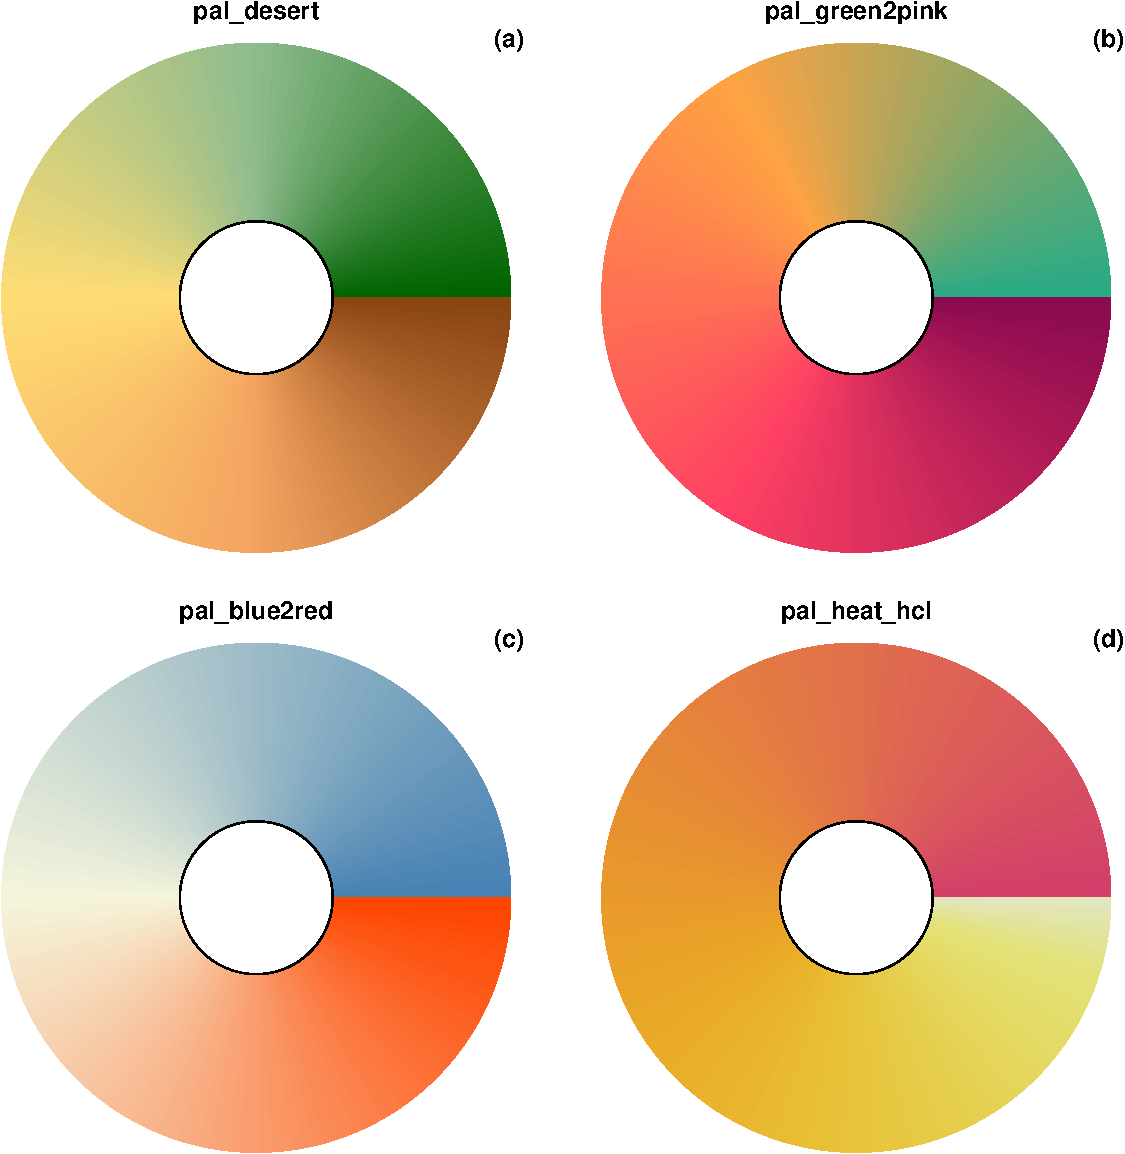
\includegraphics[width=0.8\textwidth]{/home/ven037/Dropbox/R/Git/WWRGraphics/vignettes/graphics_extensions_files/figure-latex/unnamed-chunk-1-1}

\begin{Shaded}
\begin{Highlighting}[]
\DocumentationTok{\#\#\#\# }
\DocumentationTok{\#\#\#\# Second view}
\DocumentationTok{\#\#\#\# }
\FunctionTok{plot}\NormalTok{(z, }\AttributeTok{asp =} \DecValTok{1}\NormalTok{, }\AttributeTok{cex =} \FloatTok{0.7}\NormalTok{, }\AttributeTok{ann =} \ConstantTok{FALSE}\NormalTok{, }\AttributeTok{axes =} \ConstantTok{FALSE}\NormalTok{, }\AttributeTok{bty =} \StringTok{"n"}\NormalTok{, }
     \AttributeTok{ylim =} \FunctionTok{c}\NormalTok{(}\SpecialCharTok{{-}}\DecValTok{45}\NormalTok{,}\SpecialCharTok{{-}}\DecValTok{9}\NormalTok{))}
\FunctionTok{axis}\NormalTok{(}\DecValTok{1}\NormalTok{, }\AttributeTok{at =} \DecValTok{10}\SpecialCharTok{*}\NormalTok{(}\DecValTok{11}\SpecialCharTok{:}\DecValTok{16}\NormalTok{))}
\FunctionTok{axis}\NormalTok{(}\DecValTok{2}\NormalTok{, }\AttributeTok{at =} \SpecialCharTok{{-}}\DecValTok{10}\SpecialCharTok{*}\NormalTok{(}\DecValTok{5}\SpecialCharTok{:}\DecValTok{1}\NormalTok{))}
\FunctionTok{grid}\NormalTok{()}
\FunctionTok{lines}\NormalTok{(Oz, }\AttributeTok{col =}\NormalTok{ greenish)}
\FunctionTok{arrows}\NormalTok{(z, }\FunctionTok{cyc}\NormalTok{(z), }\AttributeTok{gap =} \FloatTok{0.5}\NormalTok{, }\AttributeTok{col =}\NormalTok{ blueish)}
\NormalTok{km }\OtherTok{\textless{}{-}} \FunctionTok{gcd\_km}\NormalTok{(z, }\FunctionTok{cyc}\NormalTok{(z)) }\SpecialCharTok{\%\textgreater{}\%}\NormalTok{ round}
\FunctionTok{text}\NormalTok{((z }\SpecialCharTok{+} \FunctionTok{cyc}\NormalTok{(z))}\SpecialCharTok{/}\DecValTok{2}\NormalTok{, }\AttributeTok{labels =}\NormalTok{ km, }\AttributeTok{col =} \StringTok{"red"}\NormalTok{, }\AttributeTok{family =} \StringTok{"serif"}\NormalTok{, }
     \AttributeTok{font =} \DecValTok{4}\NormalTok{, }\AttributeTok{cex =} \FloatTok{0.8}\NormalTok{)}
\FunctionTok{title}\NormalTok{(}\AttributeTok{main =} \StringTok{"Great Circle Distances"}\NormalTok{)}
\end{Highlighting}
\end{Shaded}

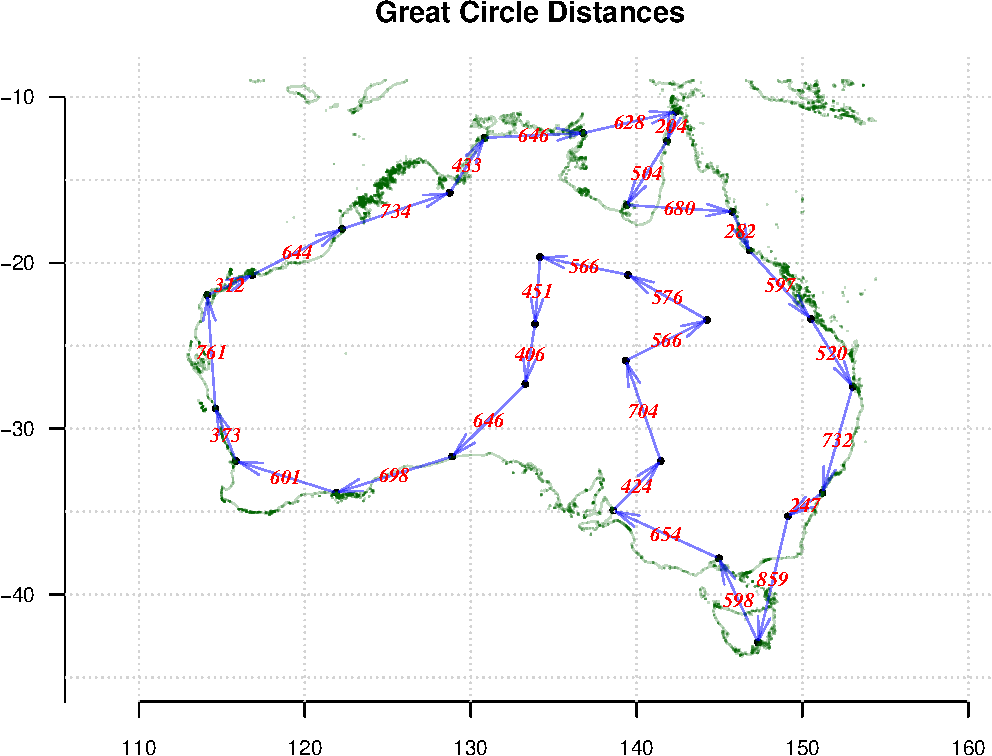
\includegraphics[width=0.8\textwidth]{/home/ven037/Dropbox/R/Git/WWRGraphics/vignettes/graphics_extensions_files/figure-latex/unnamed-chunk-1-2}

\begin{Shaded}
\begin{Highlighting}[]
\FunctionTok{library}\NormalTok{(ggplot2)}
\FunctionTok{library}\NormalTok{(ggrepel)}
\NormalTok{zfill }\OtherTok{\textless{}{-}} \ControlFlowTok{function}\NormalTok{(x) }\FunctionTok{gsub}\NormalTok{(}\StringTok{" "}\NormalTok{, }\StringTok{"0"}\NormalTok{, }\FunctionTok{format}\NormalTok{(x, }\AttributeTok{justify =} \StringTok{"right"}\NormalTok{))}
\NormalTok{ggOz }\OtherTok{\textless{}{-}} \FunctionTok{data.frame}\NormalTok{(Oz) }\SpecialCharTok{\%\textgreater{}\%} \FunctionTok{within}\NormalTok{(\{}
\NormalTok{  strip }\OtherTok{\textless{}{-}} \FunctionTok{paste0}\NormalTok{(}\StringTok{"S"}\NormalTok{, }\FunctionTok{zfill}\NormalTok{(}\FunctionTok{cumsum}\NormalTok{(}\FunctionTok{is.na}\NormalTok{(x))))}
\NormalTok{\}) }\SpecialCharTok{\%\textgreater{}\%} \FunctionTok{na.omit}\NormalTok{()}
\NormalTok{legs }\OtherTok{\textless{}{-}} \FunctionTok{data.frame}\NormalTok{(}\AttributeTok{start =}\NormalTok{ z, }\AttributeTok{end =} \FunctionTok{cyc}\NormalTok{(z), }\AttributeTok{mid =}\NormalTok{ (z }\SpecialCharTok{+} \FunctionTok{cyc}\NormalTok{(z))}\SpecialCharTok{/}\DecValTok{2}\NormalTok{, }
                   \AttributeTok{km =} \FunctionTok{round}\NormalTok{(}\FunctionTok{gcd\_km}\NormalTok{(z, }\FunctionTok{cyc}\NormalTok{(z))))}
\NormalTok{head }\OtherTok{\textless{}{-}} \FunctionTok{arrow}\NormalTok{(}\AttributeTok{length =} \FunctionTok{unit}\NormalTok{(}\FloatTok{0.0625}\NormalTok{, }\StringTok{"inches"}\NormalTok{), }\AttributeTok{angle =} \DecValTok{15}\NormalTok{, }\AttributeTok{type =} \StringTok{"closed"}\NormalTok{)}
\DocumentationTok{\#\#\#\#}
\NormalTok{g0 }\OtherTok{\textless{}{-}} \FunctionTok{ggplot}\NormalTok{(ggOz, }\FunctionTok{aes}\NormalTok{(x, y)) }\SpecialCharTok{+} 
  \FunctionTok{geom\_path}\NormalTok{(}\FunctionTok{aes}\NormalTok{(}\AttributeTok{group =}\NormalTok{ strip), }\AttributeTok{colour =}\NormalTok{ greenish) }\SpecialCharTok{+} \FunctionTok{xlab}\NormalTok{(}\StringTok{""}\NormalTok{) }\SpecialCharTok{+} \FunctionTok{ylab}\NormalTok{(}\StringTok{""}\NormalTok{) }\SpecialCharTok{+} 
  \FunctionTok{geom\_point}\NormalTok{(}\FunctionTok{aes}\NormalTok{(}\AttributeTok{x =}\NormalTok{ Longitude, }\AttributeTok{y =}\NormalTok{ Latitude), }\AttributeTok{size =} \FloatTok{0.5}\NormalTok{,}
             \AttributeTok{data =}\NormalTok{ roundTrip) }\SpecialCharTok{+} \FunctionTok{coord\_equal}\NormalTok{() }\SpecialCharTok{+} \FunctionTok{theme\_minimal}\NormalTok{() }\SpecialCharTok{+} 
  \FunctionTok{theme}\NormalTok{(}\AttributeTok{plot.title =} \FunctionTok{element\_text}\NormalTok{(}\AttributeTok{hjust =} \FloatTok{0.5}\NormalTok{), }\AttributeTok{legend.position =} \StringTok{"none"}\NormalTok{)}
\DocumentationTok{\#\#\#\#}
\NormalTok{g0 }\SpecialCharTok{+} \FunctionTok{geom\_point}\NormalTok{(}\AttributeTok{data =}\NormalTok{ roundTrip, }\FunctionTok{aes}\NormalTok{(}\AttributeTok{x =}\NormalTok{ Longitude, }\AttributeTok{y =}\NormalTok{ Latitude, }
                                      \AttributeTok{size =}\NormalTok{ Population),}
                \AttributeTok{fill =}\NormalTok{ pinkish, }\AttributeTok{colour =} \StringTok{"hot pink"}\NormalTok{, }\AttributeTok{shape =} \DecValTok{21}\NormalTok{) }\SpecialCharTok{+} 
  \FunctionTok{scale\_size\_area}\NormalTok{(}\AttributeTok{max\_size =} \DecValTok{12}\NormalTok{) }\SpecialCharTok{+}
  \FunctionTok{geom\_text\_repel}\NormalTok{(}\FunctionTok{aes}\NormalTok{(}\AttributeTok{x =}\NormalTok{ Longitude, }\AttributeTok{y =}\NormalTok{ Latitude, }\AttributeTok{label =}\NormalTok{ Locality),}
                  \AttributeTok{size =} \DecValTok{3}\NormalTok{, }\AttributeTok{data =}\NormalTok{ roundTrip) }\SpecialCharTok{+} \FunctionTok{ggtitle}\NormalTok{(}\StringTok{"Population"}\NormalTok{)}
\end{Highlighting}
\end{Shaded}

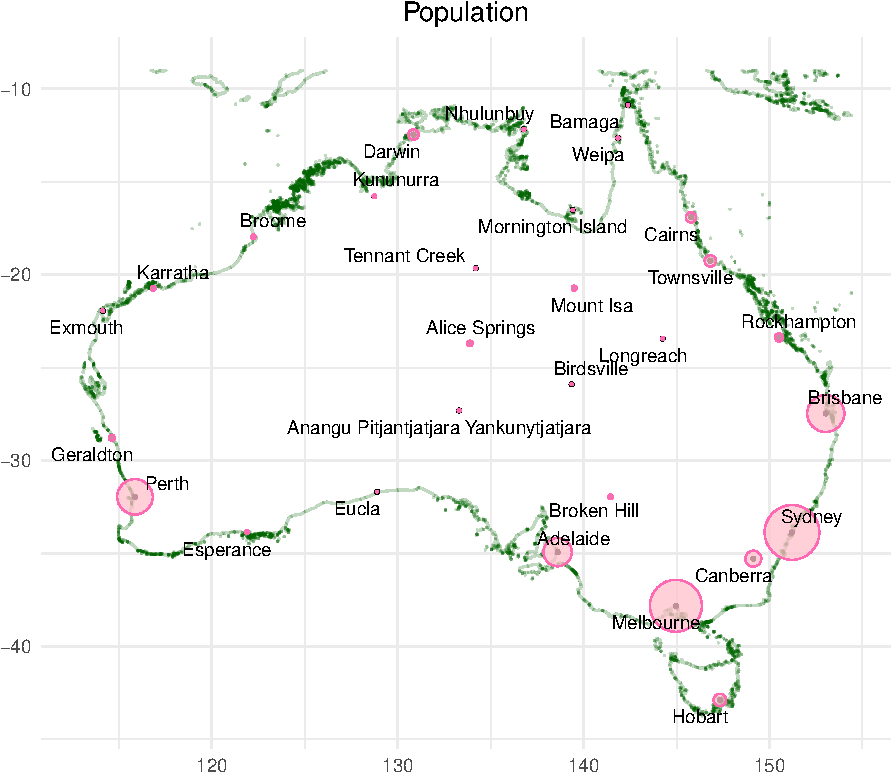
\includegraphics[width=0.8\textwidth]{/home/ven037/Dropbox/R/Git/WWRGraphics/vignettes/graphics_extensions_files/figure-latex/unnamed-chunk-2-1}

\begin{Shaded}
\begin{Highlighting}[]
\DocumentationTok{\#\#\#\#}
\NormalTok{g0 }\SpecialCharTok{+} \FunctionTok{geom\_segment}\NormalTok{(}\AttributeTok{data =}\NormalTok{ legs, }\FunctionTok{aes}\NormalTok{(}\AttributeTok{x =} \FunctionTok{Re}\NormalTok{(start), }\AttributeTok{y =} \FunctionTok{Im}\NormalTok{(start),}
                                   \AttributeTok{xend =} \FunctionTok{Re}\NormalTok{(end), }\AttributeTok{yend =} \FunctionTok{Im}\NormalTok{(end)),}
                  \AttributeTok{arrow =}\NormalTok{ head, }\AttributeTok{colour =} \StringTok{"steel blue"}\NormalTok{, }\AttributeTok{size =} \FloatTok{0.25}\NormalTok{) }\SpecialCharTok{+}
  \FunctionTok{geom\_text}\NormalTok{(}\AttributeTok{data =}\NormalTok{ legs, }\FunctionTok{aes}\NormalTok{(}\AttributeTok{x =} \FunctionTok{Re}\NormalTok{(mid), }\AttributeTok{y =} \FunctionTok{Im}\NormalTok{(mid), }
                             \AttributeTok{label =} \FunctionTok{as.character}\NormalTok{(km)), }\AttributeTok{colour =} \StringTok{"red"}\NormalTok{,}
            \AttributeTok{size =} \FloatTok{3.5}\NormalTok{, }\AttributeTok{family =} \StringTok{"serif"}\NormalTok{, }\AttributeTok{fontface =} \StringTok{"bold.italic"}\NormalTok{) }\SpecialCharTok{+} 
  \FunctionTok{ggtitle}\NormalTok{(}\StringTok{"Great Circle Distances"}\NormalTok{)}
\end{Highlighting}
\end{Shaded}

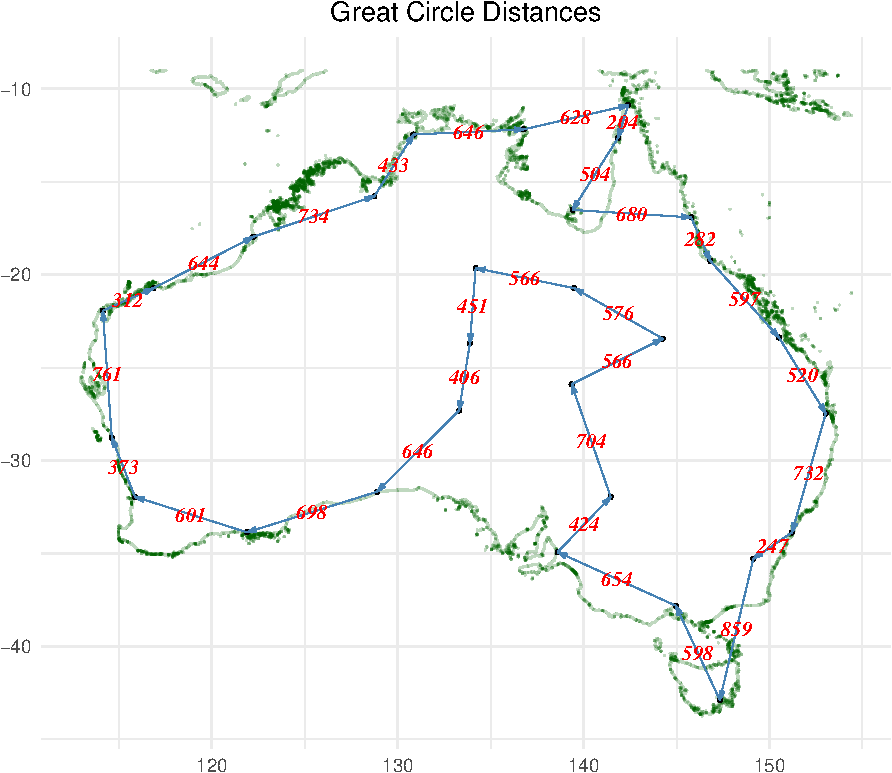
\includegraphics[width=0.8\textwidth]{/home/ven037/Dropbox/R/Git/WWRGraphics/vignettes/graphics_extensions_files/figure-latex/unnamed-chunk-2-2}

\end{document}
